%!TEX TS-program = pdflatex
%!TEX encoding = UTF-8 Unicode
\documentclass[11pt]{article}
\usepackage{acl07}
\usepackage[T1]{fontenc}
\usepackage[utf8]{inputenc}
\usepackage{times}
%\usepackage{euler}
\usepackage{graphicx}
%\usepackage{latexsym}
\usepackage{array}
%\usepackage{longtable}
\usepackage{float}
%\usepackage{natbib}
%\parskip=0pt

%\usepackage{pdfsync}
%\usepackage[
%	bookmarks,
%	bookmarksopen,
%	pdftitle=Annotation\ of\ Multiword\ Expressions\ in\ the\ Prague\ Dependency\ Treebank,
%	pdfdisplaydoctitle,
%	pdfauthor=Eduard\ Bejcek\ and\ Pavel\ Stranak,
%	pdfcreator=PdfLaTeX\ with\ Hyperref\ package,
%	colorlinks,
%	unicode,
%]{hyperref}
\usepackage{paralist} % for better itemize and enumerate
% asparaenum, inparaenum, \begin{compactenum}[{Example} a)] etc.
% Also, items can be referenced via \label{} and \ref{}
\frenchspacing
\fussy
\usepackage{amsmath}

 

\setlength\titlebox{6.5cm}    % Expanding the titlebox

\title{Annotation of Multiword Expressions in the Prague Dependency Treebank}

\author{Eduard Bejček, Pavel Straňák \protect{and} Pavel Schlesinger\\
  Institute of Formal and Applied Linguistics\\
  Charles University, Prague, Czech Republic\\
  {\tt \{bejcek,\,stranak,\,schlesinger\}@ufal.mff.cuni.cz}}  

\date{}

\begin{document}

\maketitle

\begin{abstract}
In this article we want to demonstrate that annotation of multiword expressions in the Prague Dependency Treebank is a well defined task,  
% in theory as well as in practice
that it is useful as well as feasible, and that we can achieve good consistency of such annotations in terms of inter-annotator agreement. We show a way to measure
agreement for this type of annotation. We also argue that some automatic pre-annotation is possible and it does not damage the results. 
%We use subtrees of the tectogrammatical tree structures of the Prague dependency treebank to represent the multiword expressions.

%We show that the lexico-semantic annotation\footnote{``word-sense identification'' means almost the same, but it implies ``word'' as the basic unit. We believe this view is incorrect, thus we prefer term ``lexico-semantic annotation'', that 'zduraznuje' \textit{lexeme} as the basic unit.} is necessary part of deeper treebank annotation. Further we present our methodology and subsequently preliminary results of annotation of vanilla texts, statically pre-annotated texts and compare these to preliminary results of our target annotation that includes dynamic pre-annotation based on lexemes' tree structures. Based on these data we show that our pre-annotation is justified and its benefits far outweigh its drawbacks. 

% TODO vypichnout, co je tedy cilem, ze je to ta t-anotace (a nikoli autoanotace -- takto negativne to vsak nepsat)

\end{abstract}


%%%%%
\section{Motivation} 
\label{sec:motiv}

Various projects involving lexico-semantic annotation have been ongoing for many years. 
Among those there are the projects of word sense annotation, usually for creating training data for word sense disambiguation. However majority of these projects have only annotated very limited number of word senses (cf. Kilgarriff \shortcite{kilgarriff:1998}). Even among those that aim towards ``all words'' word-sense annotation, multiword expressions (MWE) are not annotated ade\-qua\-te\-ly (see \cite{mihalcea:1998} or \cite{hajic-cwn:04}), 
because for their successful annotation a methodology allowing identification of new MWEs during annotation is required. Existing dictionaries that include MWEs concentrate only on the most frequent ones, but we argue that there are many more MWEs that can only be identified (and added to the dictionary) by annotation.

There are various projects for identification of na\-med entities (for an overview see \cite{sevcikova:2007}). We explain below (mainly in Section~\ref{sec:intro}) why we consider named entities to be concerned with lexical meaning. At this place we just wish to recall that these projects only select some specific parts of text and provide information only for these. They do not aim for full lexico-semantic annotation of texts.

There is also another group of projects that have to tackle the problem of lexical meaning, namely treebanking projects that aim to develop a deeper layer of annotation in adition to a surface syntactic layer. This deeper layer is generally agreed to concern lexical meaning. Therefore the units of this layer cannot be words anymore, they should be \textit{lexias}. 

\textit{Lexia} is defined by Filipec and Čermák \shortcite{filipec:1986} as equivalent to a ``monosemic lexeme'' of \cite{filipec:1994} or a ``lexical unit'' of \cite{cruse:1986}: \textit{``a pair of a single sense and a basic form (plus its derived forms) with relatively stable semantic properties''}. 

We work with the Prague Dependency Treebank (PDT, see Hajič \shortcite{hajic:2005}), which has in addition to the morphemic and the surface syntactic layers also the tectogrammatical layer. The latter has been construed as the layer of the (literal) meaning of the sentence and thus should be composed of lexias (lexical units) and the relations between their occurrences.%
\footnote{With a few exceptions, such as personal pronouns (that co-refer to other lexias) or coordination heads.}

On the tectogrammatical layer only the autosemantic words form nodes in a tree (t-nodes). Synsemantic (function) words are represented by various attributes of t-nodes. Each t-node has a lemma: an attribute whose value is the node's basic lexical form.
Currently t-nodes, and consequently their t-lemmas, are still visibly derived from the morphological division of text into tokens. This preliminary handling has always been considered unsatisfactory in FGD.%
\footnote{Functional Generative Description (FGD, \cite{sgall-etal:1986,hajicova:1998}) is a framework for systematic description of a language, that the PDT project is based upon. In FGD units of the t-layer are construed equivalently to monosemic lexemes (lexias) and are combined into dependency trees, based on syntactic valency of the lexias.}
There is a clear goal to distinguish t-lemmas through their senses, but %so far this process has only been completed for verbs and deverbative nouns and adjectives. 
this process has not been completed so far.

Our project aims at improving the current state of t-lemmas. Our goal is to assign each t-node a t-lemma that would correspond to a lexia, i.e. that would really distinguish the t-node's lexical meanings. To achieve this goal, in the first phase of the project, which we report on in this paper, we \textit{identify multiword expressions and create a lexicon of the corresponding lexias}. 
%Remaining t-lemmas of ``single-word t-nodes'' will be examined and possibly changed later. But to do that, we must finish the current phase in order to know what the remaining ``single-word'' nodes are.

% to leave out ???
%There are also other quite practical motivations for MWE annotation: If we want to identify coreference relations between for instance ``Association for Computational Linguistics'', ``ACL'', and  ``it'' in a text, we need to identify the first expression as a single unit. For some applications we might also need to know what kind of entity it is. 


%%%%%
%\section{Structure of the Paper}
%\label{sec:structure}

%In Section~\ref{sec:intro} we introduce our annotation task together with some necessary terminology. Section~\ref{sec:pdt} shows the current status of MWEs in the Prague Dependency Treebank, which we work with. Sections~\ref{sec:meth} and \ref{sec:pre} describe our methodology in more detail and Section~\ref{sec:analysis} presents some results, a way to measure agreement on our annotation, and an interpretation of our results.


%%%%%
\section{Introduction}
\label{sec:intro}
We annotate all occurrences of MWEs (including named entities, see below) in PDT 2.0. 
When we speak of {\bf multiword expressions} we mean ``idiosyncratic interpretations that cross word boundaries'' \newline\cite{sag:2002}. We understand multiword expressions as \textit{a type of lexias}.
%, i.e. ``the conjunction of the lexical form and the individual meaning'' \cite{filipec:1994}.
% TODO Nasledujici vetu rozvest, rozdelit na vic, zduraznit, ze prirazujeme typ.
We distinguish also a special type of MWEs, for which we are mainly interested in its type, rather than individual lexias, during the annotation: {\bf named entities (NE)}.\footnote{NEs can in general be also single-word, but in this phase of our project we are only interested in multiword expressions, so when we say NE in this paper, we always mean multiword.} 
%
Treatment of NEs together with other MWEs is important, because syntactic functions
%dependencies 
are more or less arbitrary inside a NE (consider an address with phone numbers, etc.) and so is the assignment of semantic roles.
%tectogrammatical functors. 
That is why we need each NE to be combined into a single node, just like we do it with MWEs in general. 

%Having said that in the case of NEs we care mostly for their type, we do not mean that in the future we do not want to have more information on the individual entities and possibly include them in the lexicon. Even individual names or addresses can (and should) be understood as lexias (lexical units). It is however not feasible to do this manually.
%% TODO Rozvest nasledujici vetu
%Besides, it is an excellent IR challenge to retrieve appropriate information
%% TODO NAPRIKLAD which should be appended to the lexicon entry.
%% This information varies for particular types of NE.
%for each type of NEs (see for instance \cite{feng:2006}) and
%% It is desirable to
%keep this information up to date, where needed (e.g. for persons).

For the purpose of annotation we have built a repository of lexias corresponding to MWEs, which we call SemLex. We have built it using entries from some existing dictionaries and it is being enriched during the annotation in order to contain every lexia that was annotated. We explain this in detail in Section~\ref{sec:meth:semlex}. 

%Various projects involving lexico-semantic annotation have been ongoing for many years. Majority of these however only annotated very limited number of word senses. Even among those that aimed towards ``all words'' word sense annotation, MWE were usually disregarded. Reason for this is, that these projects were annotations of plain text and so the units they work on are words. These are usually not involved in the question of What is a lexical meaning? What is a unit on the level of lexical meaning? And what level is that?

%There is also second group of projects that have to tackle the problem of lexical meaning, namely treebanking projects that aim to develop a deeper layer of annotation in addition to the surface syntactic layer. This deeper layer is mostly agreed to be the layer of lexical meaning. Therefore the units of this layer cannot be the words anymore, they should be lexias (ref.). %upravit (oslabit)


%%%%%
\section{Current state of MWEs in PDT 2.0}
\label{sec:pdt}
%
%\subsection{Multiword Expressions}
%\label{sec:pdt-mwe}

During the annotation of valency that is a part of the tectogrammatical layer of PDT 2.0  the t-lemmas that correspond to lexias have been basically identified for all the verbs and some nouns and adjectives.
The resulting valency lexicon is called PDT-VALLEX \cite{hajic:2003} and we can see it as a repository of lexias based on verbs, adjectives and nouns in PDT that have valency.
%
\footnote{It is so because in PDT-VALLEX valency is not the only criterion for distinguishing frames (=meanings). Two words with the same morphological lemma and valency frame are assigned two different frames if their meaning differs. Thus the PDT-VALLEX frames correspond to lexias.} 

This is a starting point for having t-nodes corresponding to lexias. However in the current state it is not fully sufficient even for verbs, mainly because parts of MWEs are not joined into one node. Parts of frames marked as idiomatic are still represented by separate t-nodes in a tectogrammatical tree. Verbal phrasemes are also split into 2 nodes, where the nominal part is governed by the verb. Non-verbal idioms have not been annotated at all. 

%[[!!! doplnit informaci o seznamových strukturách s kořenem \#Idph či \#Forn.]]
%Below we give two examples of the current state: an idiom meaning ``in a blink (of an eye)'' -- literally ``*what not-see'' (Figure \ref{fig:co-nevidet}) and a named entity (a name of a person) -- Václav Klaus (Figure \ref{fig:klaus}).
Below we give an example of the current state: an idiom meaning ``in a blink (of an eye)'' -- literally ``*what not-see'' (Figure \ref{fig:co-nevidet}).

\begin{figure}[htbp]
   \centering
   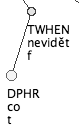
\includegraphics[width=.7in]{co-nevidet.png} 
   \caption{``Co nevidět'' (in a blink)}
   \label{fig:co-nevidet}
\end{figure}
%
%\begin{figure}[htbp] %  figure placement: here, top, bottom, or page
%   \centering
%   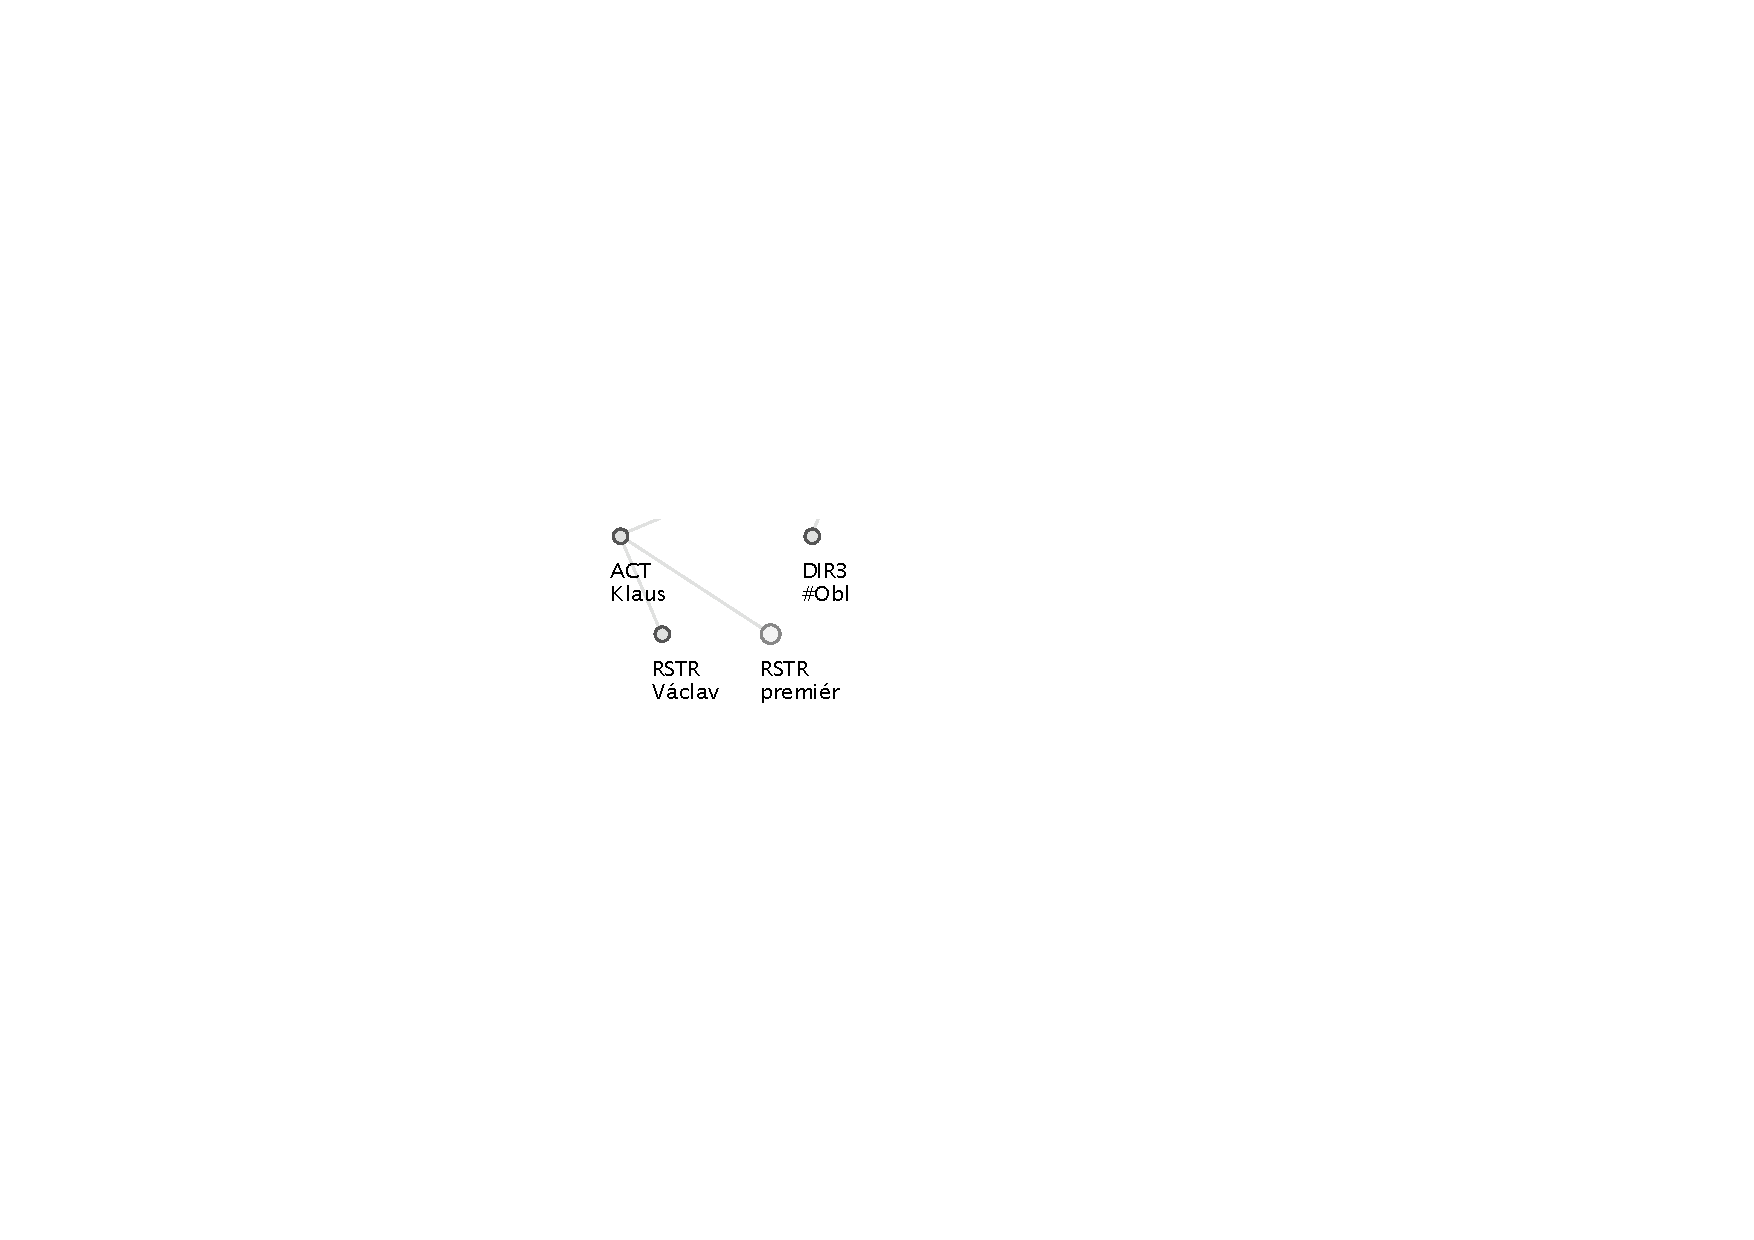
\includegraphics[width=1.5in]{Klaus.pdf} 
%   \caption{``The prime minister Václav Klaus''}
%   \label{fig:klaus}
%\end{figure}

%

%%%%%
\section{Methodology}
\label{sec:meth}

\subsection{Building SemLex}
\label{sec:meth:semlex}
Each entry we add into SemLex is considered to be a {\bf lexia}. 
We have also added 9 special entries to identify NE types, so we do not need to add the expressions themselves.
%These generic entries are ``a~name of a person or an animal'', ``institution'', ``location'', ``other object'' (used for names of books, units of measurement, biological names of plants and animals), ``address'', ``time'', ``bibliographic entry'', ``foreign expression'' and ``other entity''. 
These types are derived from NE classification by \cite{sevcikova:2007}.
%
Some frequent names of persons, institutions or other objects (e.g.~film titles) are being added into SemLex during annotation (while keeping the information about a NE type), because this allows for their following occurrences to be pre-annotated automatically (see Section~\ref{sec:pre}). For others, like addresses or bibliographic entries, it makes but little sense, because they most probably will not reappear during the annotation. 

Currently (for the first stage of lexico-semantic annotation of PDT) SemLex contains only lexias corresponding to MWEs. Its base has been composed of MWEs extracted from Czech WordNet \cite{smrz:03}, Eurovoc \cite{eurovoc:07} and SČFI \cite{cermak:1988}.%
\footnote{Slovník české frazeologie a idiomatiky (Dictionary of Czech Phraseology and Idiomatics)} 
%For the explanation of our use of the SČFI subset see point \ref{pre-hnatkova} in Section~\ref{sec:pre} below. 
Currently there are over 30,000 multi-word lexias in SemLex and more are being added during annotations.

%In the current ``compiled'' SemLex there are many collocations that can hardly be considered lexias. However, these frequently reoccurring collocations are pragmatically quite useful and it may be good to identify them, too.\footnote{We would like to mark these entries in SemLex at some point, so that we know these in fact are not lexias and we do not attempt to create a single t-node for them, when they are annotated.} The most important thing is to ensure that they are annotated consistently. They can be useful for machine translation, because, e.g., for those collocations that were extracted from Czech WordNet, there are at our disposal their translations into English (CWN). For the collocations that come from Eurovoc we have even translations into all languages of the European Union.

The entries added by annotators must be lexias as defined above. Annotators define their ``sense'' informally (as much as possible) and we extract an example of usage and the basic form from the annotation automatically. The ``sense'' information shall be revised by a lexicographer, based on annotated occurrences.


\subsection{Annotation}
\label{sec:meth:annot}

PDT 2.0 uses PML \cite{pajas:2005}, \newline{}which is an application of XML that utilises a stand-off annotation scheme. We have extended the PDT-PML with a new schema for so-called s-files. We use these files to store all of our annotation without altering the PDT itself.
These s-files are very simple: basically each of them consists of a list of s-nodes. Each s-node corresponds to an occurrence of a MWE and it is composed of a link to the entry in SemLex and a list of identifiers of t-nodes that correspond to this s-node.

Our annotation program reads in a tectogrammatical representation (t-file) and calls TrEd \cite{pajas:tred} to generate plain text. This plain text (still linked to the tectogrammatical representation) is presented to the annotator. While the annotator marks MWEs already present in SemLex or adds new MWEs into SemLex, tree representations of these MWEs extrac\-ted from underlying t-trees are added into their SemLex entries via TrEd scripts. 

%These tree representations are quite simple: for each node in a MWE we only record its t-lemma and its father's ID.


%%%%%
\section{Pre-annotation}
\label{sec:pre}
Because MWEs tend to occur repeatedly in a text, we have decided to test pre-annotation both for the speed improvement and for improving the consistency of annotations. 
%We work o
On the assumption that {\it all occurrences of a MWE share the same tree structure}, while there are no restrictions on the surface word order other than those imposed by the tree structure itself
%
% pre-annotation types
%W
we have decided to employ four types of pre-annotation:

\begin{asparaenum}[A)]
\item \label{pre-hnatkova}External pre-annotation provided by our colleague (see Hnátková \shortcite{hnatkova:2002}). With each MWE a set of rules is associated that limits possible forms and surface word order of parts of a MWE. This approach was devised for corpora that are not syntactically annotated.
\item \label{pre-static}Our one-time pre-annotation with those lexias from SemLex that were already used in annotation, and thus have a tree structure as a part of their entry.
\item \label{pre-on-load}Dynamic pre-annotation as in \ref{pre-static}, only with the SemLex entries that have been recently added by the annotator. 
\item \label{pre-on-annot}When an annotator tags an occurrence of a MWE in the text, other occurrences of this MWE in the article are identified automatically.%
%
\footnote{This is exactly what happens:
\begin{inparaenum}[1)]
\item Tree structure of the selected MWE is identified via TrEd
\item The tree structure is added to the lexeme's entry in SemLex
\item All the sentences in the given file are searched for the same MWE using its tree structure (via TrEd)
\item Other occurrences returned by TrEd are tagged with this MWE's ID, but these occurrences receive an attribute ``auto'', which identifies them (both in the s-files and visually in the annotation tool) as annotated automatically.
\end{inparaenum}
} % end footonote
\end{asparaenum}

(\ref{pre-hnatkova})~was executed once for all of the PDT. (\ref{pre-static})~is performed each time we merge lexias added by annotators into the main SemLex. We carry out this annotation in one batch for all PDT files remaining to annotate. (\ref{pre-on-load})~should be done for each file while it is being opened in LexemAnn GUI. 
(\ref{pre-on-annot})~happens each time the annotator adds a new lexia into SemLex and uses it to annotate an occurrence in the text. In subsequent files instances of this lexia are already annotated in step (\ref{pre-on-load}), and later even in (\ref{pre-static}).
%, when the lexia (lexicon entry) is merged into the main SemLex. 
 
%We have currently performed double blind annotation of a part of data without pre-annotation (\ref{pre-static}) and (\ref{pre-on-load}). We also have smaller samples annotated without any pre-annotation and only with pre-annotation (\ref{pre-hnatkova}). Analysis of this data is necessary  to show that our assumption is correct and all the occurrences of a lexia share the same tree structure. Then we can safely add remaining pre-annotation steps. Provided the inter-annotator agreement is good enough we can also stop our current (rather expensive and time consuming) practice of double annotation of each file and comparing the annotations. 

% SPOJIT !!!

After the pilot annotation without pre-annotation (\ref{pre-on-annot})  we have compared instances of the same tags and found that 10.5\% of repeated lexias happened to have two different trees. After closer examination this 10.5\% group is negligible because these cases are caused by ellipses, variations in lexical form such as diminutives etc., or wrong lemmatisation, rather than inconsistencies in the tree structure. These cases show us some issues of PDT 2.0, for instance:
\begin{compactitem}
\item \textit{jižní $\times$ Jižní Korea} [southern $\times$ South Korea] -- wrong lemmatisation
\item \textit{obchodní ředitel $\times$ ředitelka} [managing director -- man $\times$ woman] -- in future these should have one t-lemma and gender should be specified by an attribute of a t-node.
\end{compactitem}

We have not fo\-und any case that would show that there is such a MWE that its structure cannot be represented by a single tectogrammatical tree. 1.1\% of all occurences were not connected graphs, but this happened due to errors in data and to coordination. This corroborates our assumption that (disregarding errors) all occurrences of a MWE share the same tree structure. As a result, we started storing the tree structures in the SemLex entries and employ them in pre-annotation (\ref{pre-on-annot}). This also allows us to use pre-annotations (\ref{pre-static}) and (\ref{pre-on-load}), but we have decided not to use them at the moment, in order to be able to evaluate each pre-annotation step separately. Thus the following section reports on the experiments that employ pre-annotation (\ref{pre-hnatkova}) and (\ref{pre-on-annot}).


%%%%%
\section{Analysis of Annotations}
\label{sec:analysis}
Two annotators already started to use (and test) the tool we have developed.
They both have got the same texts. The text is generated from the t-trees and presented as a plain text with pre-annotated words mark\-ed by colour labels. Annotators add their tags in the form of different colour labels and they can delete the pre-annotated tags. 
%Since the units we want to annotate
%are t-nodes originated from groups of tokens, they had to annotate
%approximately 17,000 of t-nodes out of 20,000 of tokens of raw text. 
In this experiment data consists of approx. 120,000 tokens that correspond to 100,000 t-nodes.
Both annotators have marked about 15,200 t-nodes (\textasciitilde 15\%) as parts of MWEs. annotator $A$ %Vimmrova
 has grouped them into 7,263 MWEs and annotator $B$ %Sidak
  into 6,888. So the average length of a MWE is 2.2 t-nodes.

The ratio of general named entities versus SemLex lexias was 52:48 for annotator $A$ and 49:51 in case of annotator $B$. Annotator $B$ used 10\% more lexias than annotator $A$ (3,279 and 3,677), while they both used almost the same number of NEs. Some comparison is in the Table 1. %\ref{tab:anot}.

\begin{table}[h]
\begin{footnotesize}
\begin{center}
  \begin{tabular}{|l|r|r|}
\hline
type of MWE&$A$&$B$\\
\hline
SemLex lexias&3,677&3,279\\
Named Entities&3,553&3,587\\
- person/animal&1130&1137\\
- institution&842&772\\
\hline
\end{tabular}
\end{center}
\caption{Annotated instances of significant types of MWEs}
\end{footnotesize}
\label{tab:anot}
\end{table}

Both annotators also needed to add missing entries to the originally compiled SemLex or to edit existing entries. annotator $A$ added 722 entries while the annotator $B$ added 861. They modified 796 and 809 existing entries, respectively.


\subsection{Inter-anntator Agreement}
\label{agreement}

In this section our primary goal is to assess whether with our current methodology we produce reliable annotation of MWEs. To that end we measure the amount of inter-annotator agreement that is above chance. There are, however, a few sources of complications in measuring this agreement:
\begin{asparaitem}
	\item 
	Each tag of a MWE identifies a subtree of a tectogrammatical tree (represented on the surface by a set of marked words). This allows for partial agreement of tags at the beginning, at the end, but also in the middle of a surface interval (in a sentence).
	\item
	A disagreement of the annotators on the tag is still an agreement on the fact that this t-node is a part of a MWE and thus should be tagged. This means we have to allow for partial agreement on a tag.
	\item
	There is not any clear upper bound as to how many (and how long) MWEs are there in texts. 
	\item 
	There is not a clear and simple way to estimate the amount of the agreement by chance, because it must include the partial agreements mentioned above.
\end{asparaitem}

Since we want to keep our agreement calculation as simple as possible but we also need to take into account the problems above, we have decided to start from $\pi$ as defined in \cite{artstein:2007} and to make a few adjustments to allow for types of partial agreement and estimated maximal agreement.


Because we do not know how many MWEs there are in our texts, \textit{we need to calculate the agreement over all t-nodes}, rather than the t-nodes that ``should be annotated''. This also means, that the theoretical maximal agreement (upper bound) $U$, cannot be 1. If it was 1, it would be saying that all nodes are part of a MWE. 

Since we know that $U < 1$ but we do not know it's exact value, we use the \textit{estimated upper bound} $\widehat{U}$ (see Equation \ref{eq-upper-bound}). Because we calculate $\widehat{U}$ over all t-nodes, we need to account not only for agreement on tagging a t-node, but also for agreement, that the t-node is not a part of a MWE, therefore it is not tagged.%
\footnote{If we did not do this, there would be no difference between t-nodes, that were not tagged (annotators agreed they are not a part of a MWE) and the t-nodes that one annotator tagged and the other did not (i.e. they disagreed).}
%

If $N$ is the number of all t-nodes in our data and $n_{A \cup B}$ is the number of t-nodes annotated by at least one annotator, then we estimate $\widehat{U}$ as follows:
\vspace{-6pt}
\begin{equation}
\label{eq-upper-bound}
\widehat{U} = \frac{n_{A \cup B}}{N} + 0.052 \cdot \frac{N - n_{A \cup B}}{N}= 0.215
\end{equation}
\vspace{-12pt}

The weight $0.052$ used for scoring the t-nodes that were not annotated is explained below. Because $\widehat{U}$ includes all the disagreements of the annotators, we believe that the real upper bound $U$ lies somewhat below it and the agreement value 0.215 is not something that should (or could) be achieved. This is however based on the assumption that the data we have not yet seen have similar ratio of MWEs as the data we have used.

To account for partial agreement we divide the t-nodes into 5 classes $c$ and assign each class a weight $w$ as follows: 

\begin{compactenum}[$c1$]
\item
If the annotators agree on the exact tag from SemLex, we get maximum information: $w = 1$
\item
If they agree, that the t-node is a part of a NE or they agree it is a part of some lexia from SemLex, but they do not agree which NE or which lexia, we estimate we get about a half of the information compared to $c1$: $w = 0.5$
\item
If they agree that the t-node is a part of a MWE, but disagree whether a NE or a lexia from SemLex, it is again half the information compared to $c2$, so $w = 0.25$
\item
If they agree that the t-node is not a part of a MWE, $w = 0.052$. This low value of $w$ accounts for frequency of t-nodes that are not a part of a MWE, as estimated from data: Agreement on not annotating provides the same amount of information as agreement on annotating, but we have to take into account higher frequency of t-nodes that are not annotated: 

\vspace{-10pt}
\begin{small}
  \begin{align*}
  c4 &= c3 \cdot \frac{\sum annotated}{\sum not\ annotated}
       &= 0.25 \cdot \frac{12797}{61433} \approx 0.052
  \end{align*}
  \end{small}
\vspace{-10pt}
\item
If the annotators do not agree whether to annotate a t-node or not, $w = 0$. 
\end{compactenum}
The number of t-nodes ($n$) and weights $w$ per class $c$ are given in Table~2. %\ref{tab-agreement}

\begin{table}[H]
\begin{tiny}
\begin{center}
 \begin{tabular}{|l|c|c|c|c|c|}
\hline
&\multicolumn{4}{c|}{Agreement} & Disagreement\\
\cline{2-6}
&\multicolumn{3}{c|}{Agreement on annotation} & Not annotation &  \\
\cline{2-5}
&\multicolumn{2}{c|}{Agreement on NE / lexia} &&&\\
\cline{2-3}
&Full agreement &&&&\\
\cline{1-6}
class $c$& 1 & 2 & 3 & 4 & 5\\
\cline{1-6}
t-nodes $n$& 10,527 & 2,365 & 389 & 83,287 & 3,988\\
\cline{1-6}
weight $w$ & 1 & 0.5 & 0.25 & 0.052 & 0 \\
\hline
\end{tabular}
\end{center}
\caption{The agreement per class and the associated weights}
\end{tiny}
\label{tab-agreement}
\end{table}


Now that we have estimated the upper bound of agreement $\widehat{U}$ and the weights $w$ for all t-nodes we can calculate our weighted version of $\pi$:

$$\pi_w = \frac{A_o - A_e}{\widehat{U} - A_e}$$

$A_o$ is the observed agreement of annotators and $A_e$ is the agreement expected by chance (which is similar to a baseline). $\pi_w$ is thus a simple ratio of our observed agreement above chance and maximum a\-greement above chance.

Weights $w$ come into account in calculation of $A_o$ and $A_e$.

We calculate $A_o$ by multiplying the number of t-nodes in each category $c$ by that category's weight $w$, summing these 5 weighted sums and dividing this sum of all the observed agreement in the data by the total number of t-nodes:
$A_o = \frac{1}{N} \sum_{c =1}^{5} n_c w_c = 0.160$.

$A_e$ is the probability of agreement expected by chance over all t-nodes. This means it is the sum of the weighted probabilities of all the combinations of all the tags that can be obtained by a pair of annotators. Every possible combination of tags (including not tagging a t-node) falls into one of the categories $c$ and thus gets the appropriate weight $w$.
%\begin{compactitem}
%\item
%If there is an agreement on a tag, we are in $c_1$ (and $w_1 = 1$).
%\item
%When there are two tags but not identical, we are in $c_2$ or $c_3$. This depends on whether there is an agreement on choosing the same type of a SemLex entry: NE or lexia.
%\item
%An agreement on not annotating is in a class $c_4$.
%\item
%A disagreement on whether to annotate falls into the class $c_5$.
%\end{compactitem}
%
Calculating the value of $A_e$ depends not only on values of $w$ (see Table 2),
% \ref{tab-agreement}
 but also on the fact that SemLex is composed of 9 entries for NE types and over 30,000 entries for individual lexias. Based on this we have obtained $A_e = 0.047$.


The resulting $\pi_w$ is then
\vspace{-5pt} 
$$\pi_w = \frac{A_o - A_e}{\widehat{U} - A_e} = \frac{0.160 - 0.047}{0.215 - 0.047} = 0.6760$$


When we analyse the cases of disagreement and partial agreement we find that most of it has to do with SemLex lexias rather than NEs. This is mostly due to imperfectness of the dictionary and its size (annotators could not explore each of almost 30,000 of SemLex entries). Our current methodology, which relies too much on searching the SemLex, is also to blame. This should, however, improve by employing pre-annotation (\ref{pre-static}) and (\ref{pre-on-load}). 

%\begin{compactitem}
%\item 
One more reason for disagreement consists in the fact that there are cases, for which non-trivial knowledge of the world is needed: ``Jang Di Pertuan Agong Sultan Azlan Šáh, the sultan of the state of Perak, [\kern 2pt \ldots] flew back to Perak.'' Is ``Sultan Azlan Šáh'' still a part of the name or is it (or a part of it) a title?
%\item 

The last important reason of disagreement is simple: both annotators identify {\em the same} part of text as MWE instances, but while searching the SemLex they choose different lexias as the tags. This can be rectified by:
	\begin{compactitem}
		\item Removing duplicate entries from SemLex (currently there are many close identical entries originating from Eurovoc and Czech WordNet).
		\item Imploring improved pre-annotation \ref{pre-static} and \ref{pre-on-load}, as mentioned above.
	\end{compactitem}
%\end{compactitem}
%\medskip

%We have recently begun annotations of pre-annota\-ted data (type \ref{pre-hnatkova}). If we may infer from such small data (319 lexias), this type of pre-annotation slightly helps on SemLex entries (it was the object of pre-annotation, from 34.7\% to 36.5\%) and slightly spoils the NE agreement (from 71.8\% to 67.1\%). Generally, on all lexias, it slightly improves agreement (from 58.2\% to 60.1\%). Speed improvement was quite noticeable, because vast majority of pre-annotated tags might be left untouched by annotators.


% k PI:
% nase Max. je zalozene na predpokladu, ze data budou nadale podobne a anotatori nezacnou naraz anotovat vyrazne vic. 
% Max. je stanoveno tak, ze za predpokladu vyse anotator nemuze (a ani nema) Max. dosahnout. Jelikoz jde o prunik vsech anotovanych uzlu, jsou v nem i chyby (v neshodach), ty ale kompenzuji pripadne uzly, ktere ani jeden neidentifikoval, ale meli.

\section{Conclusion}

We have annotated multi-word lexias and named entities in a part of PDT 2.0. We use tectogrammatical tree structures of MWEs for the automatic pre-annotation. In the analysis of inter-annotator agreement we show that a weighted measure that accounts for partial agreement as well as the estimation of maximal agreement is needed. 

The resulting $\pi_w = 0.6760$ is statistically significant and should gradually improve as we clean up the annotation lexicon, more entries can be pre-annotated automatically, and further types of pre-annotation are employed.

%The metodology of MWE annotation we developed enables precise pre-annotation by automatically extracted tectogramatical tree structures. We have shown that this pre-annotation does improve annotation speed and should improve also agreement. Initially only manual annotation will become more automatic and our pre-annotation procedures will mark more occurances. This leaves the annotator only to decide weather this meaning is correct or not.

\section{Acknowledgement}

This work has been supported by grants 1ET2011205\-05 of Grant Agency of the Academy of Science of the Czech Republic, projects MSM0021620838 and LC536 of the Ministry of Education and 201/05/H014 of the Czech Science Foundation.


\bibliographystyle{acl}
%\bibliographystyle{plainnat}
%\newcommand{\bibfont}{\small}
\begin{small}
\bibliography{Bibliografie}
\end{small}
\end{document}
